\def\CTeXPreproc{Created by ctex v0.2.14, don't edit!}\documentclass[11pt]{article}
\usepackage{geometry}
\geometry{letterpaper}

\usepackage{graphicx}
\usepackage{amssymb}
\usepackage{epstopdf}
\usepackage{natbib}
\usepackage{amssymb,amsmath}
\usepackage{listings}
\usepackage[final]{pdfpages}
\usepackage[framed,numbered,autolinebreaks,useliterate]{ctextemp_mcode}
\usepackage{ctextemp_tikz-uml}
\usepackage{tikz}
\usepackage{subfig}
\usetikzlibrary{mindmap}

\lstset{language=matlab}
\lstset{breaklines}
\lstset{extendedchars=false}
\DeclareGraphicsRule{.tif}{png}{.png}{`convert #1 `dirname #1`/`basename #1 .tif`.png}

%\title{Title}
%\author{Name 1, Name 2}
%\date{date}

\begin{document}


\def\CTeXPreproc{Created by ctex v0.2.14, don't edit!}
\thispagestyle{empty}

\begin{center}

\includegraphics[width=5cm]{ETHlogo.eps}

\bigskip


\bigskip


\bigskip


\LARGE{ 	Lecture with Computer Exercises:\\ }
\LARGE{ Modelling and Simulating Social Systems with MATLAB\\}

\bigskip

\bigskip

\small{Project Report}\\

\bigskip

\bigskip

\bigskip

\bigskip


\begin{tabular}{|c|}
\hline
\\
\textbf{\LARGE{A Generalized Model for Peer Review:}}\\
\textbf{\LARGE{Design and Implementation}}\\
\\
\hline
\end{tabular}
\bigskip

\bigskip

\bigskip

\LARGE{Xiang Gao}



\bigskip

\bigskip

\bigskip

\bigskip

\bigskip

\bigskip

\bigskip

\bigskip

Zurich\\
Dec 2011\\

\end{center}



\newpage

%%%%%%%%%%%%%%%%%%%%%%%%%%%%%%%%%%%%%%%%%%%%%%%%%

\newpage
\section*{Agreement for free-download}
\bigskip


\bigskip


\large We hereby agree to make our source code for this project freely available for download from the web pages of the SOMS chair. Furthermore, we assure that all source code is written by ourselves and is not violating any copyright restrictions.

\begin{center}

\bigskip


\bigskip


\begin{tabular}{@{}p{3.3cm}@{}p{6cm}@{}@{}p{6cm}@{}}
\begin{minipage}{3cm}

\end{minipage}
&
\begin{minipage}{6cm}
\vspace{2mm} \large Xiang Gao

\vspace{\baselineskip}

\end{minipage}
&
\begin{minipage}{6cm}

\end{minipage}
\end{tabular}


\end{center}
\newpage

%%%%%%%%%%%%%%%%%%%%%%%%%%%%%%%%%%%%%%%

% IMPORTANT
% you MUST include the ETH declaration of originality here; it is available for download on the course website or at http://www.ethz.ch/faculty/exams/plagiarism/index_EN; it can be printed as pdf and should be filled out in handwriting
% 
\includepdf[pages={1}]{declare.pdf}

%%%%%%%%%% Table of content %%%%%%%%%%%%%%%%%

\tableofcontents

\newpage

%%%%%%%%%%%%%%%%%%%%%%%%%%%%%%%%%%%%%%%

\section{Abstract}

\section{Introduction and Motivations}

\section{Six Building Blocks for Modeling Peer Review}

\begin{tikzpicture}
\begin{umlpackage}{Common}
\umlclass{Scientist}{
  id  \\ intelligence 
}{
  produce\_paper(Producer) : Paper\\
  submit\_paper(Submitter)
}

\umlclass[y=-3]{Paper}{
  id \\ quality
}{}

\umlclass[y=-7]{Journal}{
  id \\ impact
}{
  review\_paper(Reviewer)
}

\umlclass[x=5,y=-3]{World}{
  Scientist \\ Journal
}{
  simulate\_world(Simulator)
}

\umlinterface[x=5,y=-7]{Simulator}{}{
  simulate(World)
}

\umlinterface[x=10,y=0]{Producer}{}{
  produce(Scientist)
}

\umlinterface[x=10,y=-3]{Submitter}{}{
  submit(Paper)
}

\umlinterface[x=10,y=-7]{Reviewer}{}{
  review(Journal, Paper)
}

\end{umlpackage}
\end{tikzpicture}

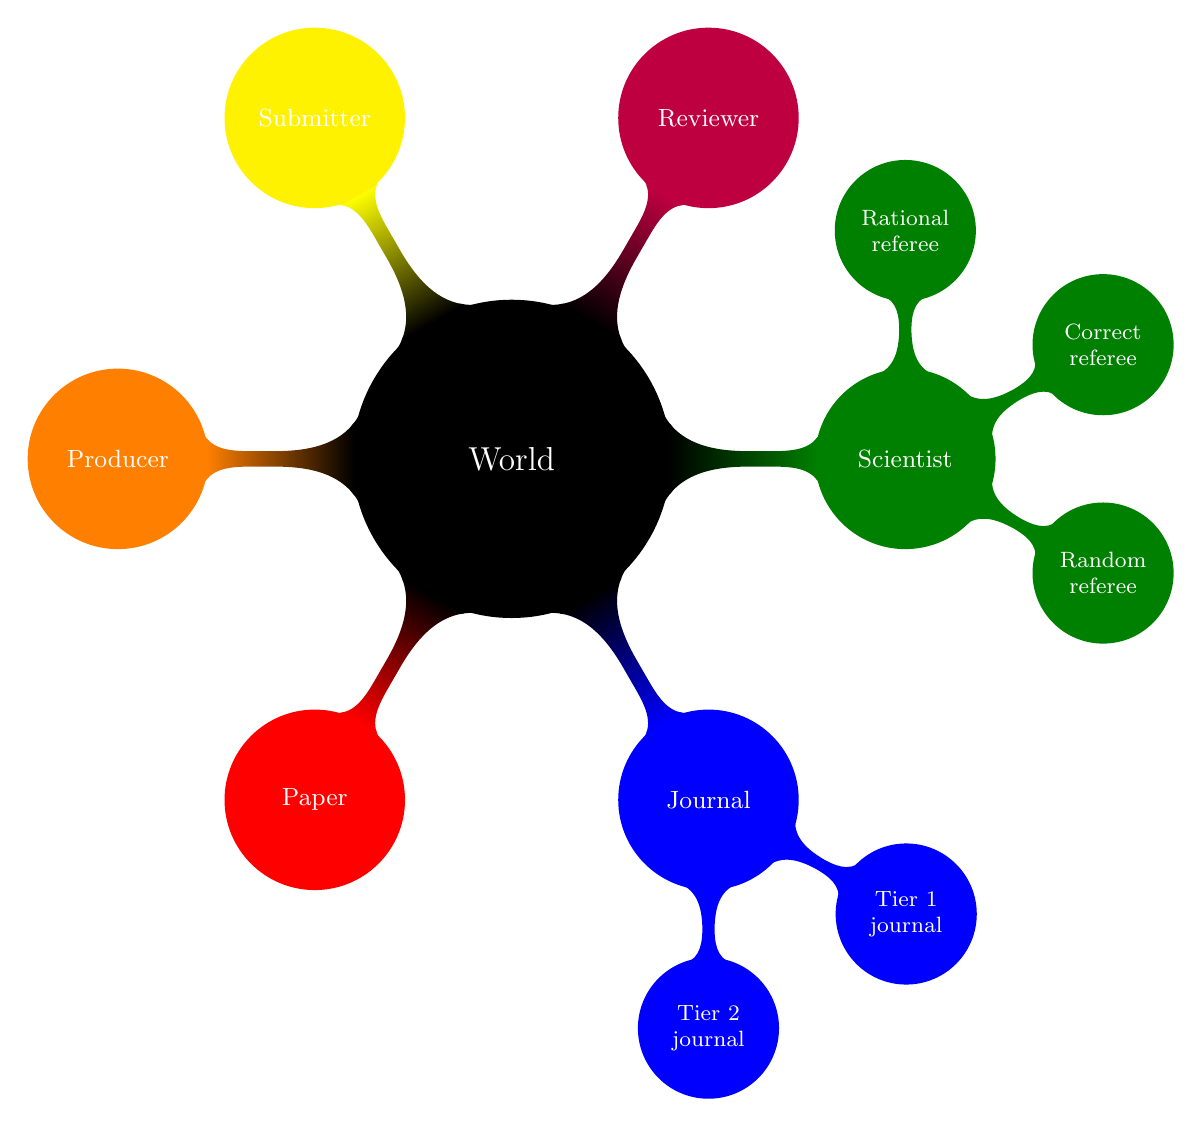
\begin{tikzpicture}
  \path[mindmap,concept color=black,text=white]
    node[concept] {World}
    [clockwise from=0]
    child[concept color=green!50!black] {
      node[concept] {Scientist}
      [clockwise from=90]
        child { node[concept] {Rational referee} }
        child { node[concept] {Correct referee} }
        child { node[concept] {Random referee} }
    }
    child[concept color=blue] {
    node[concept] {Journal}
    [clockwise from=-30]
      child { node[concept] {Tier 1 journal} }
      child { node[concept] {Tier 2 journal} }
    }
    child[concept color=red] { node[concept] {Paper} }
    child[concept color=orange] { node[concept] {Producer} }
    child[concept color=yellow] { node[concept] {Submitter} }
    child[concept color=purple] { node[concept] {Reviewer} };
\end{tikzpicture}

\section{Implementation}

\section{Simulation Results and Discussion}

\begin{figure}
    \centering
    \subfloat[][]{\resizebox{7cm}{!}{\includegraphics{../figure/Thurner/avg_quality_100_0_0.eps}}}
    \qquad
    \subfloat[][]{\resizebox{7cm}{!}{\includegraphics{../figure/Thurner/accept_quality_100_0_0.eps}}}
    \caption{Here are the first two figures of a continued figure.}
    \label{fig:cont}
\end{figure}

\begin{figure}
    \centering
    \subfloat[][]{\resizebox{7cm}{!}{\includegraphics{../figure/Thurner/avg_quality_90_0_10.eps}}}
    \qquad
    \subfloat[][]{\resizebox{7cm}{!}{\includegraphics{../figure/Thurner/accept_quality_90_0_10.eps}}}
    \caption{Here are the first two figures of a continued figure.}
    \label{fig:cont}
\end{figure}

\begin{figure}[!h]
\begin{center}
\resizebox{10cm}{!}{\includegraphics{../figure/Thurner/no_network_comparison.eps}}
\caption{Trapezoidal map to x-monotone pieces}
\end{center}
\end{figure}

\begin{figure}[!h]
\begin{center}
\resizebox{10cm}{!}{\includegraphics{../figure/Thurner/network_comparison.eps}}
\caption{Trapezoidal map to x-monotone pieces}
\end{center}
\end{figure}

\begin{figure}[!h]
\begin{center}
\resizebox{10cm}{!}{\includegraphics{../figure/Thurner/journal_comparison.eps}}
\caption{Trapezoidal map to x-monotone pieces}
\end{center}
\end{figure}

\section{Summary and Outlook}

\section{References}

\section{\texttt{Journal.m}}

\lstinputlisting{../../code/OO/common/World.m}
\lstinputlisting{../../code/OO/common/Simulator.m}
\lstinputlisting{../../code/OO/common/Scientist.m}
\lstinputlisting{../../code/OO/common/Journal.m}
\lstinputlisting{../../code/OO/common/Paper.m}
\lstinputlisting{../../code/OO/common/Producer.m}
\lstinputlisting{../../code/OO/common/Submitter.m}
\lstinputlisting{../../code/OO/common/Reviewer.m}

\lstinputlisting{../../code/OO/example/ThurnerModel.m}
\lstinputlisting{../../code/OO/example/ThurnerWorld.m}
\lstinputlisting{../../code/OO/example/ThurnerSimulator.m}
\lstinputlisting{../../code/OO/example/ThurnerScientist.m}
\lstinputlisting{../../code/OO/example/GaussianProducer.m}
\lstinputlisting{../../code/OO/example/NaiveSubmitter.m}
\lstinputlisting{../../code/OO/example/RandomReviewer.m}
\end{document}
